% Romer (2012), Problem 6.10 (pp. 308--309): solution only, the statement is not reproduced (CLAUDE.md).
% Every formula and number below is re-checked by check-6-10-6-7.py in this folder.
\problema{Romer 6.10}{Menu costs and multiple equilibria}{pp.~308--309}{Romer \S6.6--6.7}

\noindent Variables are logs. All firms face the same $p^*$, so a firm that pays the fixed cost $Z$
sets $p_i=p^*$ and one that does not keeps $p_i=0$. Firms are atomistic: one firm's choice moves
neither $f$ nor $p$, $y$ or $p^*$. Throughout, $\phi>0$ (the condition in Romer's footnote~19 for the
flexible-price equilibrium to be stable) and $m'\neq0$ (with $m'=0$ no firm has a reason to move).

\parte{a}
\passo{Eliminate $y$ from the optimal price}{Put aggregate demand $y=m'-p$ into $p^*=p+\phi y$:
\[ p^*=p+\phi(m'-p)=\phi m'+(1-\phi)\,p . \]
A firm's desired price is a weighted average of money and the price level, with weight $1-\phi$ on what the other firms charge.}
\passo{Impose $p=fp^*$ and solve for $p^*$}{Substituting $p=fp^*$,
\[ p^*=\phi m'+(1-\phi)fp^* \;\Longrightarrow\; p^*\bigl[1-(1-\phi)f\bigr]=\phi m' \;\Longrightarrow\; p^*=\frac{\phi m'}{D(f)},\qquad D(f)\equiv1-(1-\phi)f . \]
$D$ is linear in $f$ with $D(0)=1$ and $D(1)=\phi>0$, so $D>0$ on $[0,1]$ and the division is legitimate.}
\passo{Price level and output}{From $p=fp^*$ and $y=m'-p$,
\[ p=\frac{f\phi m'}{1-(1-\phi)f},\qquad y=m'-\frac{f\phi m'}{D(f)}=m'\,\frac{1-(1-\phi)f-\phi f}{D(f)}=m'\,\frac{1-f}{1-(1-\phi)f} . \]
Checks: $f=0$ gives $p=0$, $y=m'$, $p^*=\phi m'$ (output absorbs the whole shock); $f=1$ gives $p=p^*=m'$ and $y=0$ (neutrality). In between, $\partial y/\partial f=m'\,[-D(f)+(1-f)(1-\phi)]/D(f)^2=-\phi m'/D(f)^2$: each extra adjuster pushes output toward its flexible-price level.}

\parte{b}
\passo{The incentive function}{A firm that keeps $p_i=0$ loses $K(0-p^*)^2$ relative to a firm at $p^*$; a firm that adjusts loses nothing before paying $Z$. The gross gain from adjusting, as a function of the fraction $f$ of \emph{other} firms that adjust, is therefore
\[ G(f)\equiv Kp^{*2}=\frac{K\phi^2m'^2}{\bigl[1-(1-\phi)f\bigr]^2},\qquad G(0)=K\phi^2m'^2,\qquad G(1)=\frac{K\phi^2m'^2}{\phi^2}=Km'^2 . \]}
\passo{Slope and curvature}{Write $G=K\phi^2m'^2D^{-2}$ with $D'(f)=-(1-\phi)$. By the chain rule,
\[ \begin{aligned} G'(f)&=-2K\phi^2m'^2D^{-3}D'(f)=\frac{2K\phi^2m'^2(1-\phi)}{D(f)^3},\\ G''(f)&=-6K\phi^2m'^2(1-\phi)D^{-4}D'(f)=\frac{6K\phi^2m'^2(1-\phi)^2}{D(f)^4}\ \ge0 . \end{aligned} \]
As $D>0$, $\operatorname{sign}G'=\operatorname{sign}(1-\phi)$. \emph{Real rigidity, $\phi<1$:} $G$ is strictly increasing and convex, rising from $K\phi^2m'^2$ to $Km'^2$; price adjustments are strategic complements. \emph{Real flexibility, $\phi>1$:} $G$ is strictly decreasing and convex, falling from $K\phi^2m'^2$ to $Km'^2$; adjustments are strategic substitutes. At $\phi=1$, $p^*=m'$ whatever the others do and $G\equiv Km'^2$.}

\begin{center}\begin{minipage}{\linewidth}\centering
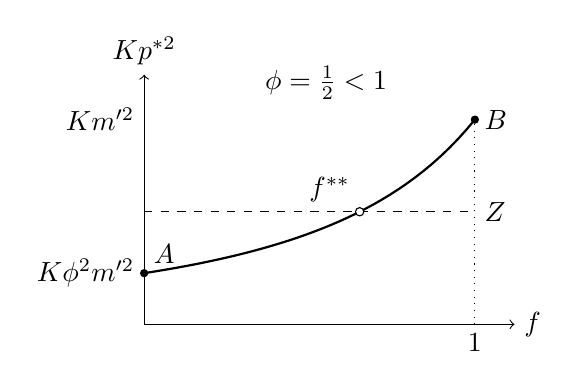
\begin{tikzpicture}[x=4.2cm,y=2.6cm]
  \draw[->] (0,0)--(1.12,0) node[right]{$f$};
  \draw[->] (0,0)--(0,1.22) node[above]{$Kp^{*2}$};
  \draw[thick,domain=0:1,samples=40] plot (\x,{0.25/((1-0.5*\x)^2)});
  \draw[dashed] (0,0.55)--(1,0.55) node[right]{$Z$};
  \draw[dotted] (1,0)--(1,1);
  \node[left] at (0,0.25){$K\phi^2m'^2$}; \node[left] at (0,1){$Km'^2$}; \node[below] at (1,0){$1$};
  \fill (0,0.25) circle (1.5pt) node[above right]{$A$};
  \fill (1,1) circle (1.5pt) node[right]{$B$};
  \draw[fill=white] (0.6516,0.55) circle (1.5pt) node[above left]{$f^{**}$};
  \node at (0.55,1.18){$\phi=\frac12<1$};
\end{tikzpicture}\qquad
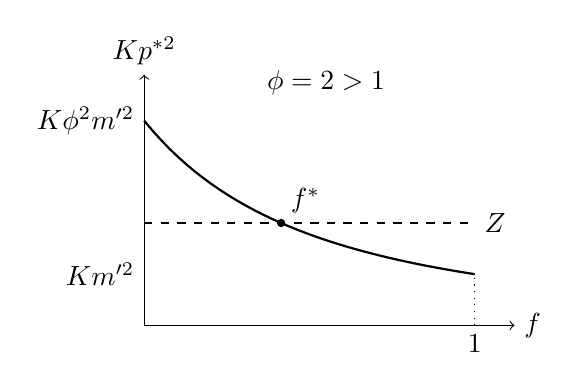
\begin{tikzpicture}[x=4.2cm,y=0.65cm]
  \draw[->] (0,0)--(1.12,0) node[right]{$f$};
  \draw[->] (0,0)--(0,4.9) node[above]{$Kp^{*2}$};
  \draw[thick,domain=0:1,samples=40] plot (\x,{4/((1+\x)^2)});
  \draw[dashed] (0,2)--(1,2) node[right]{$Z$};
  \draw[dotted] (1,0)--(1,1);
  \node[left] at (0,4){$K\phi^2m'^2$}; \node[left] at (0,1){$Km'^2$}; \node[below] at (1,0){$1$};
  \fill (0.4142,2) circle (1.5pt) node[above right]{$f^{*}$};
  \node at (0.55,4.75){$\phi=2>1$};
\end{tikzpicture}\par\smallskip
{\small $G(f)=Kp^{*2}$ with $K=m'=1$. Left, $Z=0.55$: equilibria at $A$ ($f=0$), $B$ ($f=1$) and the
unstable $f^{**}\approx0.652$. Right, $Z=2$: the unique equilibrium $f^*=\sqrt2-1\approx0.414$.}
\end{minipage}\end{center}

\parte{c}
\passo{What an equilibrium is}{Each firm takes $f$ as given; it adjusts if $G(f)>Z$, stays if $G(f)<Z$, and may do either if $G(f)=Z$. A configuration is an equilibrium when no firm wants to switch:
\[ \begin{aligned} f=1 \text{ is an equilibrium} &\iff G(1)\ge Z \iff Z\le Km'^2,\\ f=0 \text{ is an equilibrium} &\iff G(0)\le Z \iff Z\ge K\phi^2m'^2,\\ f\in(0,1) \text{ is an equilibrium} &\iff G(f)=Z , \end{aligned} \]
since in the interior case every firm is indifferent, so any split between adjusters and non-adjusters is a best response.}
\passo{Both corners at once}{Both $f=0$ and $f=1$ are equilibria iff $K\phi^2m'^2\le Z\le Km'^2$. This interval is non-empty iff $\phi^2\le1$, i.e.\ (as $\phi>0$) iff $\phi\le1$, and has positive length iff $\phi<1$. Answer: \emph{yes, exactly when $\phi<1$ and $Z\in[K\phi^2m'^2,\,Km'^2]$.} For $Z$ strictly inside, $G$ crosses $Z$ once more, at $f^{**}=\bigl(1-\phi|m'|\sqrt{K/Z}\bigr)/(1-\phi)$ (solve $G(f)=Z$ as in the last step); this third equilibrium is unstable, since just above it $G>Z$ and more firms want to adjust, and just below it $G<Z$ and adjusters want to stop. At $\phi=1$ the interval shrinks to $Z=Km'^2$, where $G\equiv Z$ and every $f\in[0,1]$ is an equilibrium.}
\passo{Neither corner}{Neither is an equilibrium iff $G(1)<Z$ and $G(0)>Z$, i.e.\ $Km'^2<Z<K\phi^2m'^2$, which is non-empty iff $\phi>1$. Answer: \emph{yes, exactly when $\phi>1$ and $Z\in(Km'^2,\,K\phi^2m'^2)$.}}
\passo{The interior equilibrium when neither corner works}{For $\phi>1$, $G$ is continuous and strictly decreasing with $G(0)>Z>G(1)$, so exactly one $f^*\in(0,1)$ has $G(f^*)=Z$. Since $D>0$,
\[ \begin{aligned} \frac{K\phi^2m'^2}{D(f^*)^2}=Z &\iff D(f^*)=\phi|m'|\sqrt{K/Z} \iff 1+(\phi-1)f^*=\phi|m'|\sqrt{K/Z}\\ &\iff f^*=\frac{\phi|m'|\sqrt{K/Z}-1}{\phi-1}, \end{aligned} \]
and $0<f^*<1\iff1<\phi|m'|\sqrt{K/Z}<\phi\iff Km'^2<Z<K\phi^2m'^2$, the same interval. At $f^*$, $|p^*|=\sqrt{Z/K}$: adjusters move by exactly the amount that makes the menu cost worth paying. With $D^*\equiv D(f^*)$ and $1-f^*=(\phi-D^*)/(\phi-1)$, output is $y^*=m'(\phi-D^*)/[(\phi-1)D^*]$, strictly between $0$ and $m'$ because $1<D^*<\phi$: money is partly neutral. The equilibrium is stable (for $f>f^*$, $G<Z$ and adjusters prefer to stay; for $f<f^*$, $G>Z$ and more firms adjust), and with $\phi>1$ the equilibrium is always unique, because $G$ is strictly monotone and the two corner conditions are incompatible.}

\begin{center}\small
\begin{tabular}{@{}lccc@{}}
\toprule
 & $Z<\min\{G(0),G(1)\}$ & $Z$ between $G(0)$ and $G(1)$ & $Z>\max\{G(0),G(1)\}$\\
\midrule
$\phi<1$ & only $f=1$ & $f=0$ and $f=1$ (and $f^{**}$ if $Z$ is interior) & only $f=0$\\
$\phi>1$ & only $f=1$ & only $f^*$ (stable) & only $f=0$\\
\bottomrule
\end{tabular}
\end{center}

\intuicao{With $\phi<1$ the desired price $p^*=\phi m'+(1-\phi)p$ leans on the others' prices. If nobody else moves, a firm's optimal change is only $\phi m'$, worth $K\phi^2m'^2$; if everybody moves it is the full $m'$, worth $Km'^2$. A menu cost between the two makes both outcomes self-fulfilling: the same nominal shock leaves the economy either rigid, with $y=m'$ (a recession when $m'<0$), or flexible, with $y=0$. Each firm's price change helps the others through aggregate demand, an externality it ignores, which is why Ball and D.~Romer (1991) read nominal rigidity as a coordination failure (Romer \S6.8). Real rigidity therefore does double duty: it shrinks the private gain from adjusting when others stay put, and it makes adjustment decisions complements. With $\phi>1$ the others' adjustment shrinks a firm's own desired change, decisions are substitutes, the equilibrium is unique, and an intermediate menu cost yields partial adjustment.}
\armadilha{(1) Letting the deviating firm's own choice move $p$ and $p^*$: with a continuum of firms its deviation has measure zero, so $p^*$ is evaluated at the others' $f$. (2) Writing the corner conditions with strict inequalities only: an indifferent firm may do either, so the intervals are closed and $f=1$ survives at $Z=Km'^2$. (3) Reading $G(0)<G(1)$ as multiplicity for every $Z$: it needs $Z\in[K\phi^2m'^2,Km'^2]$, and outside that interval the equilibrium is unique even with $\phi<1$. (4) Treating only expansions: everything depends on $m'^2$ and $|m'|$, so a contraction is the mirror image.}
\refbib{Romer (2012), \S6.6--6.7 (pp.~275--286): the incentive to adjust, real rigidity and eq.~(6.58); \S6.8 (from p.~286): coordination failure. Ball and D.~Romer (1991), ``Sticky Prices as Coordination Failure,'' \emph{American Economic Review} 81, 539--552.}
\checado{\texttt{check-6-10-6-7.py} re-derives $p^*$, $p$, $y$, $G$, $G'$, $G''$ and $f^*$ with sympy, and with $K=m'=1$ confirms the interval $[0.25,1]$ and three equilibria at $Z=0.55$ for $\phi=\frac12$ ($f^{**}=0.6516$), and the unique $f^*=y^*=\sqrt2-1$ at $Z=2$ for $\phi=2$, by scanning $G(f)-Z$ on a grid; the same scan confirms both interval claims, and uniqueness whenever $\phi>1$, on a grid of $Z$ for $\phi\in\{0.5,0.75,1.5,2\}$. The solution manual agrees on every part; it states the intervals with strict inequalities and does not solve for the interior equilibrium.}
